\documentclass[conference]{IEEEtran}

\usepackage{cite}
\usepackage{amsmath,amssymb,amsfonts}
\usepackage{algorithmic}
\usepackage{graphicx}
\usepackage{textcomp}
\usepackage{xcolor}
\usepackage{csquotes}
\usepackage[hidelinks]{hyperref}

\def\BibTeX{{\rm B\kern-.05em{\sc i\kern-.025em b}\kern-.08em
  T\kern-.1667em\lower.7ex\hbox{E}\kern-.125emX}}
\begin{document}

\title{Decentralized Access Control}%*\\

\author{
  \IEEEauthorblockN{Heinrich Lorenz}
  Karlsruhe, Germany \\
  lorenz.heinrich@student.kit.edu
}

\maketitle

\begin{abstract}
  In the era of digitalization, online collaboration, and artificial intelligence data plays a crucial role.
  However, the practices this data is managed often disregard the user's privacy, and power over this data is increasingly accumulated by large enterprises.
  This work aims to provide an understanding of the domain of data management, particularly focusing on access control for privacy-sensitive data.
  It analyzes the status quo in which individuals find themselves, introduces a theoretical decentralized access control model, and discusses the potential improvements decentralized technologies can offer.
  Furthermore, it explores the role of decentralized access control within the broader context of data sovereignty identifying its contributions and dependencies.
\end{abstract}

\section{Introduction}
Data sharing is a key element in our everyday lives.
Driven by cloud applications, wearables, the digitalization of the health sector, and many more, the amount of generated personal and privacy-sensitive data is rapidly increasing.
And indeed, the applications of shared personal data cannot be denied.
Patients may want as much data for their diagnosis to be used as possible while also wanting their medical records to be available for others \cite{hollis_share_2016}.
Athletes may want to share fitness data with service providers for analysis, and users of the web may want their data to be used for a personalized experience \cite{nasir_council_nodate}.
However, if individuals do not want to publicly share their data, some kind of mechanism is required allowing them to specify \textit{who} gets access to \textit{what} data \textit{when}.

Current industry standards rely on centralized authorization and authentication mechanisms acting on behalf of a user to manage data access. \cite{hardt_oauth_2012,noauthor_googles_nodate}
These practices demand individuals to trust in the correctness of these services while most of the time no effort is made to provide insight into the actual processes.
Additionally, due to the assumption that the service providers are a part of the user's trusted domain, the data is often visible in clear to them, leading to increasing privacy concerns.
This situation has led to emerging voices questioning who should wield ultimate power over data and how the users' ability to manage their data without relying on third parties can be enhanced \cite{noauthor_w3f_nodate}.
In essence, this describes the idea of data sovereignty where self-sovereign individuals with the ability to manage their identity and data without trusted intermediates can interact and share data while preserving their privacy \cite{ernstberger_sok_2023}.

In this work, the status quo of access control systems currently used in web-based services will be analyzed while also formulating the key aspects of an access control system.
After clarifying the shortcomings current practices suffer from, an alternative model based on decentralized technologies will be introduced.
By the example of the decentralized access control system Droplet, concrete aspects of decentralized access control will be discussed in further detail, concluding with an evaluation of the contributions of decentralized access control to the idea of data sovereignty.

\section{Access Control}
In the context of web services, the term \textit{access control} refers to \enquote{the process of granting or denying specific requests to [\dots] obtain and use information and related information processing services [\dots]}. [reference] % // TODO: add a citation
Traditionally, in the realm of access control, an individual who owns the data subject to access control is designated as the \textit{resource owner}, while the entity seeking access is commonly referred to as the \textit{client}.
Moreover, the infrastructure housing the protected resources is denoted as the \textit{resource server}.

\subsection{Access Control in Web 2.0}
Web 2.0, as we know it today, heavily relies on contributing, creating, and collaborating on various platforms \cite{community_web_2019}.
As a consequence, there is a demand for systems supporting fine-grained access control to the resources generated and owned by users.

A web service (client) requesting access to an access-restricted resource hosted on a resource server can access the resource by using the resource owner's credentials.
Using this method to grant access comes with several issues.
First, the resource owner has no option but the update his credentials if he wants to revoke the granted access.
Second, by disclosing the credentials to the resource server, the client gets access to all resources hosted on that server and third, the compromisation of that client results in a compromisation of the resource owner's credentials and therefore all of the resources of the user hosted on the resource server.
Analyzing these issues, one can conclude that the desirable properties of an access control system include

%//TODO: maybe inline?
\begin{enumerate}
  \item \textbf{Fine-Grained Access Scope:} Resource owners should be able to specify to which resources they grant access at what point in time.
  \item \textbf{Individual Access:} Resource owners should be able to independently grant access to different clients.
  \item \textbf{Revocability of Access:} Resource owners should be able to revoke granted access at any time with minimal effort.
\end{enumerate}

\subsubsection*{OAuth}
To address the challenges the above-described naive authorization approach entails, the OAuth protocol delineates an authorization flow for access control systems outlining the process by which clients can request access to protected resources while enabling resource owners to fulfill these requests without disclosing their credentials.
The protocol introduces an \textit{authorization server} that authenticates clients and enforces restricted access to resources on behalf of the resource owner.
The client can request access to a resource of the resource owner and by that obtain an \textit{authorization grant}.
This grant declares the client as authorized by the resource owner and enables the client to obtain an \textit{access token} from the authorization server in exchange for the authorization grant.
This token contains a set of attributes specifying to which resource the client has access to.
Using this token, the client can request the resource from the resource server, which in turn validates the access token and returns the resource in case of a valid token \cite{hardt_oauth_2012}.

\subsection{Shortcomings of Centralized Access Control}
\label{sec:shortcomings}
Access control systems based on the OAuth 2.0 framework indeed mitigate the problems introduced by the naive authorization method by separating the resource owner from the client.
The protocol allows the resource owner the individually specify which client gets access to what data when enforced by the access tokens issued by the authorization server \cite{hardt_oauth_2012}.
Thereby key aspects of an access control system are implemented including the properties defined above.

However, the centralized nature of the authorization and resource server introduces a new dimension of concerns.
Users must trust these entities to comply with the OAuth specification and effectively protect their data by prohibiting access to data from unauthorized clients.
Additionally, since the OAuth protocol builds upon trust in centralized entities, data on the resource server is not protected from the service providers violating the privacy of users and increasing the risk of data breaches.
Centralized access control systems also suffer from a single point of failure increasing the risk of unauthorized access.

Unfortunately, these concerns are not only valid in theory but regard the everyday experience of individuals using these services.
Chen, 2014 examined popular mobile apps using OAuth 2.0 and found that more than half of the examined applications implemented the OAuth 2.0 flow incorrectly, thus making the application, and consequently the data of the users vulnerable \cite{chen_oauth_2014}.
To address privacy concerns, governments are trying to protect users via regulatory frameworks raising the question of how to ensure service providers follow accordingly \cite{noauthor_general_nodate}.

\section{Decentralized Access Control}
\label{sec:decentralized_access_control}
Shortcomings in privacy have led to a call for a paradigm shift towards a \textit{user-centric} approach, as opposed to a \textit{data-centric} approach, both in technical and non-technical communities \cite{ernstberger_sok_2023, shafagh_droplet_2020}.
The primary goal of the concept of decentralized access control is to bring back the power over the data to the data owners by treating data privacy as a first-class citizen \cite{ernstberger_sok_2023}.
Decentralized access control leverages decentralized technologies, threshold cryptography, and end-to-end encryption to contribute to the realization of user-centric systems, tackling the fundamental issues centralized approaches entail.

\subsection{Definition}
Decentralized Access Control enables resource owners to verifiably share data with data consumers by specifying fine-grained access policies without exposing the data in cleartext to any third party and without the need to rely on any trusted intermediate while preserving their privacy.

\subsection{Model}
In the following, a theoretical model of decentralized access control is introduced.
This model is described not strictly, but mostly according to Ernstberger, 2023 \cite{ernstberger_sok_2023}.

\subsubsection{Entities}
The following entities are utilized:

\begin{itemize}
  \item \textbf{User:} An individual or organization that owns data that is subject to access control.
  \item \textbf{Data Consumer:} An entity that is interested in the data of a user and wants to access it.
  \item \textbf{Storage:} An abstract storage unit that stores encrypted data and is available to both the data consumer and the user.
  \item \textbf{Access Controler:} A computational node that enforces access policies on behalf of the user.
  \item \textbf{Distributed Ledger:} A distributed, append-only, and globally verifiable data structure that logs transactions.
  By utilizing proof-of-work and consensus algorithms, mutually distrustful parties manage a global state that is deemed trustworthy under specific assumptions without relying on a central trusted entity.
  A prominent illustration of this concept can be found in blockchain-based technologies \cite{zheng_overview_2017}.
\end{itemize}

\begin{figure}[htbp]
  \centering
  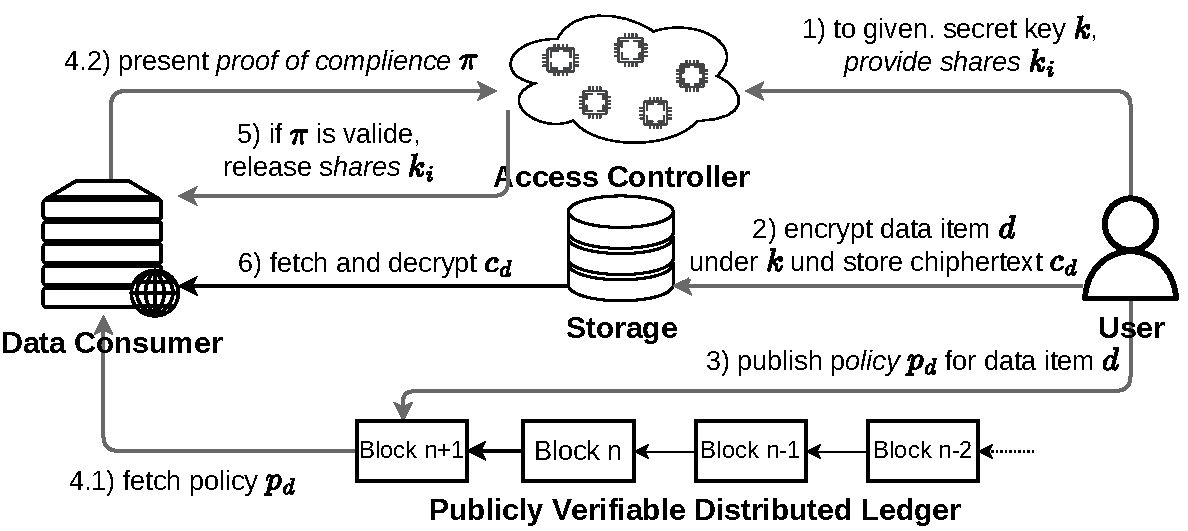
\includegraphics[width=\linewidth]{figures/decentralized_access_control.pdf}
  \caption{
    This figure illustrates the flow between the entities according to the decentralized access control model by depicting the steps and interactions required by each entity to perform authorized access. \cite{ernstberger_sok_2023}.
    In \autoref{sec:supported_actions}, the steps are elaborated in further detail.
  }
  \label{fig:decentralized_access_control}
\end{figure}

\subsubsection{Supported Actions}
\label{sec:supported_actions}
The supported actions of the decentralized access model are introduced alongside the scenario in which a user wants to share data with a data consumer.
The user achieves this by utilizing a decentralized access control system that complies with the introduced model.

\begin{enumerate}
  \item The user generates a secret key $s$ that is used for the encryption of the data item $d$, the user wants to share.
  Using a $(k,n)$ secret sharing scheme, the user generates $n$ shares from that secret such that $k$ shares are sufficient to reconstruct the secret $s$ \cite{shamir_how_1979}.
  These shares are shared with a committee of $n$ access controls where each access controller receives one share.
  \item Using the secret $s$, the user encrypts  $d$ and stores the resulting ciphertext $c_d$ in the storage.
  \item To specify the set of authorized data consumers, a policy $p_d$ is generated defining under which conditions a data consumer is authorized to access the $d$.
  This policy is then published to the ledger $L$.
  \item A data consumer that wants to access $d$, fetches $p_d$ from $L$ and calculates a cryptographic proof $\pi$, claiming him as authorized to access $d$.
  \item By presenting $\pi$ to the committee of access controllers, the data consumer requests access to $d$.
  \item Each access controller validates $\pi$ by checking it against $p_d$ published on $L$.
  If $\pi$ is valid, the access controller releases its share to the data consumer.
  \item The data consumer can reconstruct $s$ in case of $k$ access controllers releasing their share.
  Finally, the data consumer obtains $c_d$ from the storage and accesses $d$ by decrypting $c_d$ using the reconstructed secret $s$. 
\end{enumerate}

\subsection{Improvements Over Centralized Approaches}
As analyzed in \autoref{sec:shortcomings}, centralized access control falls short in respecting the users' privacy and providing reliable systems that transparently enforce access policies.
The root of these issues lies in the centralized nature of the policy-enforcing entities.

By only storing ciphertexts in storage units, the privacy violations of data breaches can be minimized ensuring data confidentiality independently from the safety of the storage system. The single point of failure the authorization server is subject to is resolved by decentralizing the policy enforcement point.
No trust in any single access controller in the committee is necessary, since the decentralized access control model tolerates $n - k$ misbehaving nodes.
Any authentication and access can be audited by the user if requested, by corresponding transactions to the ledger enabling the user to independently verify the correctness of the access control system.
Privacy for data consumers and users is provided by keeping data consumers anonymous during authentication and access unless requested by an audit.

\section{Access Policies for Time Series Data Streams}
Droplet \cite{shafagh_droplet_2020} is a decentralized access control system designed for time series data streams produced by IoT devices \cite{zhang_cloud_2015}.
It leverages end-to-end encryption access control and blockchain technology, to allow flexible data sharing of data streams from IoT owned by the resource owner without involving trusted intermediates.
Despite Droplet not relying on distributed secret management as the policy enforcement point but encrypting the key material required for decryption using the data consumers' public key, in the following, the flexible, crypto-based access policies are analyzed as an example.

Droplet uses a combination of different cryptographic concepts to ensure, that data consumers get only access to a specified set of data.
Due to the nature of time series data, time is regarded as the primary attribute for specifying access policies.
The core idea of Droplets' access policies is to serialize the data stream into time-encoded data chunks, each encrypted using a unique key assigned per chunk.
Employing binary hash trees and dual-key regression, the access policies can be encoded into a small set of keys.

\subsection{Binary Hash Tree}
Given an initial secret random seed as the root, utilizing two different hash functions $hash_l()$ and $hash_r()$, a binary hash tree can be derived to an arbitrary height.
Using a key-derivation function to generate keys from the leaves of the binary hash tree enables the user to share arbitrary intervals of key material by only sharing the corresponding inner nodes.

\subsection{Dual-Key Regression}
Key regression schemes allow the derivation of previous keys by applying the hash function successively on a given hash token \cite{fu_key_2005, shafagh_droplet_2020}.
This practically enables the sharing of decryption keys from the current time to the beginning, by providing the current hash token.
But since the all-or-none principle this method entails is not desirable in scenarios where data should only be shared from a certain point in time until now, Droplet employs a contrary hash chain enforcing a lower time-bound.
With the need to have both tokens available to derive the corresponding key, the lower time-bound can be enforced by sharing only the token from that point in time for the contrary hash chain.
Due to the pre-image resistance of hash functions, it is computationally impractical to calculate any previous hash tokens.

\begin{figure}[htbp]
  \centering
  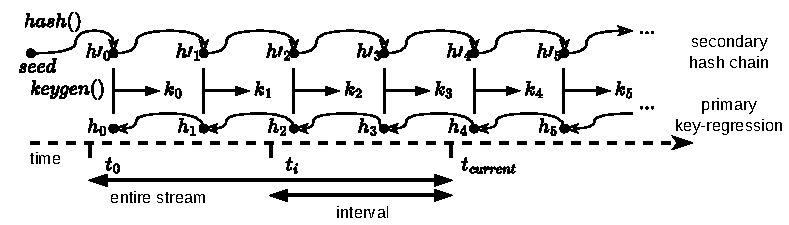
\includegraphics[width=\linewidth]{figures/dual_key_regression.pdf}
  \caption{
    This figure is inspired by Figure 4 from Shafagh, 2020 \cite{shafagh_droplet_2020} and illustrates the dual-key regression mechanism.
    It enhances traditional key regression to only calculate keys to a specified lower time-bound.
    The $keygen()$ function requires the tokens from both the primary key-regression and the secondary hash chain to derive the key $k_i$ from the time point $t_i$.
    By sharing the token $h'_i$ paired with the current token of the primary key-regression, the data consumer can calculate all keys from $t_i$ to $t_{current}$. 
  }
  \label{fig:dual_key_regression}
\end{figure}

\subsection{Access Policies}
Droplet's access policies consist of the ID of the stream subject to the policy, the public key of the data owner the user wants to share a subset of the stream with, and the specified access scope that is either an inner node from the corresponding binary hash tree or a hash token to a certain point in time if access shall be granted in subscription mode.

Droplet, as an example, provides insight into how access policies can be tailored for particular use cases.
The theoretical model of decentralized access control, as outlined in \autoref{sec:decentralized_access_control}, enables a diverse range of applications.
By providing a broad framework without delving into specific implementation details, concrete access control systems can build upon this basis while addressing the specific requirements and challenges of their respective domain.

\section{Data Sovereignty of Decentralized Access Control}
\begin{itemize}
  \item 
\end{itemize}

\bibliographystyle{IEEEtran}
\bibliography{references}

\end{document}
